\documentclass[12pt]{article}
\usepackage[utf8]{inputenc}
\usepackage[T1]{fontenc}
\usepackage{amssymb}
\usepackage{amsthm}
\usepackage{amsmath}
\usepackage{mathtools}
\usepackage{booktabs}
\usepackage{array}
\usepackage{dcolumn}
\usepackage{multirow}
\usepackage{adjustbox}
\usepackage{subfig}
\usepackage{graphicx}
\usepackage{listings}
\usepackage{natbib}
\usepackage[obeyspaces,hyphens]{url}
\usepackage{lscape}
\usepackage{nicefrac}
\usepackage{xcolor}
\usepackage{txfonts}
\usepackage{empheq}
\usepackage{fancyhdr}
\usepackage{xurl}
\usepackage{ragged2e}
\usepackage{microtype}
\usepackage{tikz}
\usetikzlibrary{arrows.meta,calc,angles,quotes,positioning}
\usepackage[
    unicode=true,
    pdfencoding=auto,
    psdextra,
    plainpages=false,
    pdfpagelabels,
    pagebackref=false,
    hyperindex,
    breaklinks=true,
    colorlinks=true,
    citecolor=black,
    linkcolor=black,
    urlcolor=blue,
    filecolor=black,
    bookmarksopen=true
]{hyperref}
\usepackage[
    a4paper,
    left=18mm,
    right=18mm,
    top=16mm,
    bottom=18mm,
    headheight=15.8pt,
    headsep=4mm,
    footskip=8mm,
    includeheadfoot
]{geometry}

%%%%%%%%%%%%%%%%%%%%%%%%%%%%%%%%%%%%%%%%%%%%%%%%%%%%%%%%%%%%%%%%%%%%%%%
\pdfstringdefDisableCommands{%
  \def\textit#1{#1}%
  \def\emph#1{#1}%
  \def\textbf#1{#1}%
  \def\\{ }%
}
%%%%%%%%%%%%%%%%%%%%%%%%%%%%%%%%%%%%%%%%%%%%%%%%%%%%%%%%%%%%%%%%%%%%%%%
\newcommand{\be}{\begin{equation}}
\newcommand{\ee}{\end{equation}}
\def\ni{\noindent}
\newcommand{\bse}{\begin{subequations}}
\newcommand{\ese}{\end{subequations}}
\newcommand{\lb}[1]{\label{#1}}
\newcommand{\dd}{{\mathrm{d}}}
\newcommand{\R}{\mathbb{R}}
\newcommand{\C}{\mathbb{C}}
\newcommand{\N}{\mathbb{N}}
\newcommand{\Z}{\mathbb{Z}}
\newcommand{\Q}{\mathbb{Q}}
\newcommand{\deri}[2]{\ensuremath{\frac{\dd #1}{\dd #2}}}

%%%%%%%%%%%%%%%%%%%%%%%%%%%%%%%%%%%%%%%%%%%%%%%%%%%%%%%%%%%%%%%%%%%%%%%
% Mathematical and didactic environments
\newtheorem{exercise}{Exercise}[section]
\newtheorem{definition}{Definition}[section]
\newtheorem{theorem}{Theorem}[section]
\newtheorem{example}{Example}[section]
\newtheorem{corollary}{Corollary}[section]
\newtheorem{proposition}{Proposition}[section]
\newtheorem{remark}{Remark}[section]

\numberwithin{equation}{section}

\pagestyle{fancy}
\fancyhf{}
\fancyhead[R]{\small\itshape\nouppercase{\leftmark}}
\fancyfoot[L]{\scriptsize Osvaldo L. Santos-Pereira --- \href{mailto:olsp@if.ufrj.br}{olsp@if.ufrj.br}}
\fancyfoot[C]{\scriptsize \thepage}
\renewcommand{\headrulewidth}{0.4pt}
\renewcommand{\footrulewidth}{0.4pt}

\urlstyle{same}

% Author block for cover page
\newcommand{\coverauthor}[4]{%
{\large\bfseries #1\par}
\vspace{0.02cm}
{\normalsize\href{mailto:#2}{#2}\par}
\vspace{0.02cm}
{\normalsize\color{blue}\url{#3}\par}
\vspace{0.02cm}
{\normalsize\itshape #4\par}
\vspace{0.8cm}
}

\long\def\coveraboutme#1{%
\vspace{0.3cm}
\begingroup
{\large\bfseries\color{black} About Me\par}
\vspace{0.18cm}
\small
\color{black!85}
\justifying
\setlength{\parindent}{18pt}
\setlength{\parskip}{3pt}
\setlength{\emergencystretch}{2em}
#1
\par
\endgroup
\vspace{0.5cm}
}

\newcommand{\sociallink}[2]{%
\noindent{\footnotesize\color{black!80} #1: \url{#2}\par}
}

\newcommand{\chaptercover}[4]{%
\begin{titlepage}
\thispagestyle{empty}
\raggedright
\setlength{\parindent}{0pt}
\vspace*{0.2cm}
{\fontsize{34}{40}\selectfont\bfseries #1\par}
\vspace{1.0cm}
{\fontsize{26}{30}\selectfont\bfseries #2\par}
\vspace{1.5cm}
\rule{\textwidth}{2.0pt}
\vspace{1.0cm}
#3
\vspace{0.3cm}
#4
\vfill
\end{titlepage}
}
%%%%%%%%%%%%%%%%%%%%%%%%%%%%%%%%%%%%%%%%%%%%%%%%%%%%%%%%%%%%%%%%%%%%%%%

\begin{document}

\chaptercover
{Quadratic Equations}
{Algebra, Geometry, Complex Roots, Tangents, and Applications}
{
\coverauthor
{Osvaldo L. Santos-Pereira}
{olsp@if.ufrj.br}
{https://ozsp12.github.io/}
{Physics Institute of Federal University of Rio de Janeiro (UFRJ)}
}
{
\coveraboutme{
\noindent
I hold a PhD in Physics from the Federal University of Rio de Janeiro (UFRJ), a Master's degree in Physics from the State University of Campinas (Unicamp), a Master's degree in Data Science and Analytics from the University of S\~ao Paulo (MBA USP-ESALQ), a postgraduate degree in Quantum Computing from SENAI-CIMATEC, and a Bachelor's degree in Physics from Unicamp.

\noindent
I am currently a Fellow Researcher at the Physics Institute of the Federal University of Rio de Janeiro (UFRJ), where I research Warp Drive Theory, Classical General Relativity, Cosmology, Econophysics, and Computational Physics. Other research interests include Wormhole Theory, Black Hole Theory, Quantum Gravity, Quantum Computing and Information, Mathematics, and Artificial Intelligence.

\noindent
I work in the private sector as a data science consultant and an artificial intelligence specialist. I conduct research projects across several industries, including education, health, medical, e-commerce, and large retail.

\vspace{0.3cm}
\sociallink{Curr\'iculo Lattes}{http://lattes.cnpq.br/6730251976463283}
\sociallink{ResearchGate}{https://www.researchgate.net/profile/Osvaldo-Santos-Pereira}
\sociallink{ORCID}{https://orcid.org/0000-0003-2231-517X}
\sociallink{Google Scholar}{https://scholar.google.com/citations?user=HIZp0X8AAAAJ&hl=en}
\sociallink{LinkedIn}{https://www.linkedin.com/in/ozsp12}
\sociallink{Substack}{https://substack.com/@olsp1982}
\sociallink{GitHub}{https://github.com/ozsp12}
\sociallink{YouTube}{https://www.youtube.com/@ozlsp12}
}
}

\tableofcontents
\newpage

%%%%%%%%%%%%%%%%%%%%%%%%%%%%%%%%%%%%%%%%%%%%%%%%%%%%%%%%%%%%%%%%%%%%%%%
\section{Introduction}

Quadratic equations occupy an unusual position in mathematics: they belong to elementary algebra, yet they already contain several ideas that reappear in more advanced subjects. Their solution requires algebraic manipulation, the distinction between reversible and nonreversible transformations, the structure of number systems, and the interpretation of polynomial zeros. Their graphs lead directly to the geometry of the parabola, conic sections, symmetry, extrema, and tangency. Their negative discriminant forces an enlargement of the real numbers to the complex numbers, while their factorization anticipates the Fundamental Theorem of Algebra. In calculus, the same polynomial becomes a first model for derivatives, tangent lines, stationary points, and optimization. For this reason, a serious treatment of quadratic equations is not merely a rehearsal of a formula; it is a compact introduction to the way algebra, geometry, analysis, and mathematical modeling interact.

The historical development of the subject is correspondingly broad. Old Babylonian mathematical texts contain procedures for problems that, in modern notation, reduce to quadratic equations, although these procedures were expressed rhetorically and were embedded in numerical and geometric problems rather than in symbolic algebra \cite{robson2008,katz2009}. Greek mathematics treated geometrically related problems through constructions and the theory later described as ``application of areas.'' In India, Brahmagupta developed explicit rules for quadratic equations in the seventh century, and later authors, including \=Sr\={i}dhara and Bh\={a}skara II, refined algebraic techniques and discussed positive, negative, and irrational quantities with a sophistication that is essential to the history of the subject \cite{plofker2009,colebrooke1817}. In the Islamic mathematical tradition, al-Khw\={a}rizm\={i}'s ninth-century treatise systematically classified linear and quadratic equations and justified their solution through geometric arguments equivalent to completing the square \cite{rosen1831,swetzkatz2011}. Renaissance and early-modern symbolic algebra, particularly the work of Vi\`ete, Girard, and Descartes, gradually produced the notation in which the modern theory is now expressed \cite{boyer2011,katz2009}.

A terminology point is worth making at the outset. In Brazilian school mathematics the quadratic formula is often called the ``Bhaskara formula.'' This name is not standard in the international literature, where \emph{quadratic formula} is the usual term, and the modern symbolic formula should not be attributed to a single author. The mathematical ideas that led to it developed across several civilizations over many centuries. Bh\={a}skara II is an important figure in this history, but Brahmagupta, al-Khw\={a}rizm\={i}, earlier Mesopotamian mathematics, and the later development of symbolic algebra are also indispensable parts of the story \cite{plofker2009,katz2009,boyer2011}.

For readers who want a strong elementary foundation, Lang's \emph{Basic Mathematics} and Gelfand and Shen's \emph{Algebra} are particularly useful because they emphasize structure rather than mechanical substitution \cite{lang1988,gelfandshen1993}. Coxeter's \emph{Introduction to Geometry} is a classical reference for geometric thinking and conics \cite{coxeter1969}. Apostol and Spivak provide rigorous transitions from elementary algebra to calculus \cite{apostol1967,spivak2008}. For historical context, Katz, Boyer and Merzbach, Robson, and Plofker give complementary accounts of the Mesopotamian, Greek, Indian, Islamic, and European traditions \cite{katz2009,boyer2011,robson2008,plofker2009}. The aim of this note is to combine these perspectives in a self-contained exposition that begins with elementary prerequisites and ends with calculus and physical applications.

%%%%%%%%%%%%%%%%%%%%%%%%%%%%%%%%%%%%%%%%%%%%%%%%%%%%%%%%%%%%%%%%%%%%%%%


\section{Review of Elementary Concepts}

Quadratic equations are elementary only in the sense that they occur early in the curriculum. A complete understanding presupposes a collection of ideas about numbers, algebraic expressions, logical equivalence, factorization, and functions. This section fixes notation and reviews those ideas in the form needed later. The emphasis is not on exhaustive treatment but on the structural facts that make the theory of quadratic equations work.

\subsection{Number systems and elementary logic}

The standard number systems used throughout this note are
\be
\N \subset \Z \subset \Q \subset \R \subset \C.
\ee
Natural numbers count discrete objects, integers allow subtraction without leaving the set, rational numbers allow quotients of integers with nonzero denominator, real numbers complete the number line, and complex numbers allow square roots of negative real numbers. The passage from one system to the next is not cosmetic: the solvability of an equation depends on the domain in which solutions are sought.

A mathematical equation is a proposition containing one or more variables. Solving an equation over a set $S$ means determining all values in $S$ that make the proposition true. Logical equivalence is therefore central. If two equations have exactly the same solution set, we write informally that one transformation is equivalent to the other. Adding the same expression to both sides and multiplying both sides by a nonzero quantity are reversible operations. Squaring both sides is not always reversible and can introduce extraneous solutions. This distinction becomes important whenever radicals or rational expressions appear.

\begin{definition}[Solution set]
Let $E(x)$ be an equation and let $S$ be a prescribed domain. The solution set is
\be
\mathcal{S}=\{x\in S:E(x)\text{ is true}\}.
\ee
\end{definition}

\begin{remark}
An equation may have different solution sets over $\R$ and $\C$. For example, an equation with a negative discriminant has no real roots but has two complex roots counted with multiplicity.
\end{remark}

\subsection{Monomials and polynomials}

A monomial in one variable has the form $a x^n$, where $a$ is a coefficient and $n$ is a nonnegative integer. A polynomial is a finite sum of monomials,
\be
P(x)=a_nx^n+a_{n-1}x^{n-1}+\cdots+a_1x+a_0,
\qquad a_n\neq 0.
\ee
Its degree is $n$. A quadratic polynomial is a polynomial of degree two. The coefficient $a_n$ is called the leading coefficient, while $a_0$ is the constant term.

Polynomial addition and multiplication remain within the set of polynomials. Division is more subtle: division by a nonzero polynomial produces a quotient and a remainder. The factor theorem states that $x-r$ divides $P(x)$ if and only if $P(r)=0$. This simple result is the algebraic bridge between roots and factorization.

\begin{theorem}[Factor theorem]
For a polynomial $P(x)$ over a field and a scalar $r$, the following statements are equivalent:
\be
P(r)=0
\qquad\Longleftrightarrow\qquad
P(x)=(x-r)Q(x)
\ee
for some polynomial $Q(x)$.
\end{theorem}

\begin{proof}
By polynomial division, $P(x)=(x-r)Q(x)+R$, where the remainder $R$ is constant. Setting $x=r$ gives $P(r)=R$. Hence $P(r)=0$ if and only if $R=0$.
\end{proof}

\subsection{Algebraic identities and factorization}

Several identities recur throughout quadratic algebra. The most important are
\bse
\begin{align}
(a+b)^2 &= a^2+2ab+b^2,\\
(a-b)^2 &= a^2-2ab+b^2,\\
(a+b)(a-b) &= a^2-b^2.
\end{align}
\ese
These formulas are not merely shortcuts for multiplication. They provide the mechanism behind completing the square, which in turn produces both the quadratic formula and the canonical form of a parabola.

A quadratic expression can sometimes be factored by inspection. For example,
\be
x^2-5x+6=(x-2)(x-3).
\ee
The factorization immediately reveals the roots. When inspection is not practical, completing the square or the quadratic formula gives a systematic method.

\subsection{Equivalent transformations of equations}

Suppose $A(x)=B(x)$. Adding the same expression $C(x)$ to both sides gives an equivalent equation. Multiplication by a nonzero constant is also reversible. Division by an expression depending on $x$ is reversible only after excluding the values for which that expression vanishes. The general principle is that every algebraic operation used in solving an equation must be checked for reversibility on the chosen domain.

Completing the square is a sequence of reversible transformations when the leading coefficient is nonzero. This fact is the logical basis of the derivation in Sec.~\ref{sec:quadratic_formula}. By contrast, replacing $A=B$ by $A^2=B^2$ yields the weaker statement $A=\pm B$, so a later verification may be required.

\subsection{Functions, zeros, and graphs}

A function $f:A\to B$ assigns to each $x\in A$ exactly one value $f(x)\in B$. The set $A$ is the domain, $B$ is the codomain, and the set of values actually assumed by the function is its image. A zero or root of $f$ is a number $r$ in the domain such that $f(r)=0$.

For a polynomial function, the equation $P(x)=0$ asks for the intersections of the graph $y=P(x)$ with the $x$-axis when real coordinates are used. This gives the first geometric interpretation of the discriminant: two real roots correspond to two intersections, a repeated root corresponds to tangency to the axis, and nonreal roots correspond to the absence of real intersections.

\begin{exercise}
Factor each polynomial whenever possible over the integers: $x^2-9$, $x^2+7x+12$, $2x^2-5x-3$, and $x^2+4$.
\end{exercise}

\begin{exercise}
Explain why the transformation $x=1\Rightarrow x^2=1$ is valid but the reverse implication is false. Identify the extra solution introduced by reversing the argument.
\end{exercise}

%%%%%%%%%%%%%%%%%%%%%%%%%%%%%%%%%%%%%%%%%%%%%%%%%%%%%%%%%%%%%%%%%%%%%%%


\section{Quadratic Equations}

The general quadratic equation is the first polynomial equation for which a complete symbolic theory can be developed with elementary tools. Its coefficients determine the number and type of roots, the geometry of its graph, its factorization, and its extremum. The theory is sufficiently simple to be explicit and sufficiently rich to illustrate several central mathematical themes.

\subsection{Historical route from problems to symbols}

Ancient quadratic problems were not written as equations in the modern sense. Mesopotamian procedures were expressed in words and often concerned lengths and areas; nevertheless, many are equivalent to solving quadratic relations \cite{robson2008}. Al-Khw\={a}rizm\={i} classified quadratic equations into separate positive-coefficient types because negative coefficients were not treated as freely as they are in modern algebra. His geometric arguments amount to completing the square \cite{rosen1831,swetzkatz2011}. Indian algebraists developed rules in a different tradition, with Brahmagupta and Bh\={a}skara II occupying prominent positions \cite{plofker2009,colebrooke1817}. Modern symbolic notation compressed these rhetorical procedures into a single equation and, eventually, a single formula.

The historical lesson is mathematical as well as cultural. The compact expression used today depends on an enlarged number system, signed coefficients, symbolic variables, and an acceptance of multiple roots. Once these conventions are in place, cases that had historically required separate verbal rules become different regimes of one algebraic object.

\subsection{Definition and standard form}

\begin{definition}[Quadratic equation]
A quadratic equation in one variable is an equation of the form
\be
ax^2+bx+c=0,
\qquad a\neq 0,
\lb{eq:quadratic_standard}
\ee
where $a$, $b$, and $c$ are coefficients in a specified number system.
\end{definition}

The requirement $a\neq0$ is essential. If $a=0$, Eq.~\eqref{eq:quadratic_standard} is linear or degenerate. Multiplying all coefficients by the same nonzero constant does not change the roots, so the triple $(a,b,c)$ represents the same equation as $(\lambda a,\lambda b,\lambda c)$ for every $\lambda\neq0$.

\subsection{Completing the square and the quadratic formula}
\label{sec:quadratic_formula}

Starting from Eq.~\eqref{eq:quadratic_standard}, divide by $a$:
\be
x^2+\frac{b}{a}x+\frac{c}{a}=0.
\ee
Move the constant term to the right-hand side,
\be
x^2+\frac{b}{a}x=-\frac{c}{a},
\ee
and add the square of half the coefficient of $x$ to both sides:
\be
x^2+\frac{b}{a}x+\frac{b^2}{4a^2}
=
\frac{b^2}{4a^2}-\frac{c}{a}.
\ee
The left-hand side is a perfect square,
\be
\left(x+\frac{b}{2a}\right)^2
=
\frac{b^2-4ac}{4a^2}.
\lb{eq:completed_square}
\ee
Taking square roots gives
\be
x+\frac{b}{2a}
=
\pm\frac{\sqrt{b^2-4ac}}{2a},
\ee
where the square root is interpreted in the appropriate number system. Hence
\be
\boxed{
x=\frac{-b\pm\sqrt{b^2-4ac}}{2a}
}.
\lb{eq:quadratic_formula}
\ee

\begin{remark}[On the name ``Bhaskara formula'']
Equation~\eqref{eq:quadratic_formula} is called the \emph{quadratic formula} in the international literature. The widespread Brazilian name ``Bhaskara formula'' recognizes an important Indian algebraic tradition, but it should not be interpreted as a historically exclusive attribution. Equivalent methods and formulas have a long history involving Mesopotamian mathematics, Brahmagupta, al-Khw\={a}rizm\={i}, Bh\={a}skara II, and later symbolic algebra \cite{katz2009,plofker2009,boyer2011}.
\end{remark}

\subsection{The discriminant and the three solution regimes}

\begin{definition}[Discriminant]
The discriminant of the quadratic polynomial $ax^2+bx+c$ is
\be
\Delta=b^2-4ac.
\lb{eq:discriminant}
\ee
\end{definition}

The sign of $\Delta$ classifies the roots over $\R$.

\begin{proposition}[Discriminant classification]
Let $a,b,c\in\R$ with $a\neq0$.
If $\Delta>0$, the equation has two distinct real roots. If $\Delta=0$, it has one repeated real root. If $\Delta<0$, it has no real roots and has two nonreal complex conjugate roots.
\end{proposition}

\begin{proof}
The conclusion follows directly from Eq.~\eqref{eq:quadratic_formula}. The quantity $\sqrt{\Delta}$ is nonzero real when $\Delta>0$, zero when $\Delta=0$, and purely imaginary up to a real factor when $\Delta<0$.
\end{proof}

\begin{table}[htbp]
\centering
\caption{Algebraic and geometric meaning of the discriminant for real coefficients.}
\begin{tabular}{@{}lll@{}}
\toprule
Condition & Roots over $\R$ & Graphical meaning \\
\midrule
$\Delta>0$ & two distinct roots & two crossings of the $x$-axis \\
$\Delta=0$ & one double root & tangency to the $x$-axis \\
$\Delta<0$ & no real roots & no intersection with the $x$-axis \\
\bottomrule
\end{tabular}
\end{table}

\begin{figure}[htbp]
\centering
\begin{tikzpicture}[scale=0.8,>=Stealth]
% Delta > 0
\begin{scope}[xshift=-6cm]
\draw[->] (-2.2,0)--(2.2,0) node[right] {$x$};
\draw[->] (0,-1.8)--(0,2.4) node[above] {$y$};
\draw[thick,domain=-1.9:1.9,samples=80] plot (\x,{0.7*\x*\x-1.1});
\fill (-1.253,0) circle (1.8pt); \fill (1.253,0) circle (1.8pt);
\node at (0,-2.25) {$\Delta>0$};
\end{scope}
% Delta = 0
\begin{scope}
\draw[->] (-2.2,0)--(2.2,0) node[right] {$x$};
\draw[->] (0,-1.8)--(0,2.4) node[above] {$y$};
\draw[thick,domain=-1.9:1.9,samples=80] plot (\x,{0.7*\x*\x});
\fill (0,0) circle (1.8pt);
\node at (0,-2.25) {$\Delta=0$};
\end{scope}
% Delta < 0
\begin{scope}[xshift=6cm]
\draw[->] (-2.2,0)--(2.2,0) node[right] {$x$};
\draw[->] (0,-1.8)--(0,2.4) node[above] {$y$};
\draw[thick,domain=-1.9:1.9,samples=80] plot (\x,{0.7*\x*\x+0.8});
\node at (0,-2.25) {$\Delta<0$};
\end{scope}
\end{tikzpicture}
\caption{Three geometric regimes of a quadratic with $a>0$. For $a<0$ the figures are reflected vertically, but the number of real roots is unchanged.}
\lb{fig:discriminant_cases}
\end{figure}

For polynomials of degree greater than two, a discriminant can also be defined. In general it is a polynomial in the coefficients that vanishes precisely when the polynomial has a repeated root over an algebraic closure. For a quadratic, this general construction reduces to Eq.~\eqref{eq:discriminant}. Thus the familiar quantity $b^2-4ac$ is the first instance of a much broader algebraic invariant.

\subsection{The parabola and the geometric meaning of the roots}

The graph of
\be
f(x)=ax^2+bx+c
\ee
is a parabola. If $a>0$, the graph opens upward and the function is convex. If $a<0$, the graph opens downward and the function is concave. The real roots are precisely the $x$-coordinates at which the graph intersects the $x$-axis. A repeated root means that the vertex lies on the axis and the graph is tangent to it.

Completing the square gives the canonical form
\be
f(x)=a\left(x+\frac{b}{2a}\right)^2-\frac{\Delta}{4a}.
\lb{eq:vertex_form}
\ee
Equation~\eqref{eq:vertex_form} already displays the axis of symmetry and the vertex without using calculus.

\begin{proposition}[Vertex]
The parabola $y=ax^2+bx+c$ has vertex
\be
\left(x_v,y_v\right)
=
\left(-\frac{b}{2a},-\frac{\Delta}{4a}\right).
\lb{eq:vertex}
\ee
\end{proposition}

\subsection{Vi\`ete--Girard relations and notable identities}

Let the roots be $x_1$ and $x_2$, counted with multiplicity. If the polynomial factors as
\be
ax^2+bx+c=a(x-x_1)(x-x_2),
\ee
then expansion gives
\be
ax^2-a(x_1+x_2)x+a x_1x_2.
\ee
Comparing coefficients yields the classical root--coefficient relations.

\begin{theorem}[Vi\`ete--Girard relations]
For $a\neq0$,
\bse
\begin{align}
x_1+x_2&=-\frac{b}{a},\lb{eq:viete_sum}\\
x_1x_2&=\frac{c}{a}.\lb{eq:viete_product}
\end{align}
\ese
\end{theorem}

In much of the international literature these are called Vi\`ete's formulas. The name Girard also appears in historical and pedagogical traditions because Albert Girard developed systematic relations between roots and coefficients in the early seventeenth century \cite{katz2009,boyer2011}.

Several useful identities follow immediately:
\bse
\begin{align}
x_1^2+x_2^2
&=(x_1+x_2)^2-2x_1x_2
=\frac{b^2-2ac}{a^2},\\
(x_1-x_2)^2
&=(x_1+x_2)^2-4x_1x_2
=\frac{\Delta}{a^2},\\
\frac{1}{x_1}+\frac{1}{x_2}
&=\frac{x_1+x_2}{x_1x_2}
=-\frac{b}{c},\qquad c\neq0.
\end{align}
\ese
The second identity shows directly that the separation between two real roots is
\be
|x_1-x_2|=\frac{\sqrt{\Delta}}{|a|}.
\lb{eq:root_separation}
\ee
Thus the discriminant controls not only whether the roots are real but also how far apart they are on the real line.

\subsection{Rational and integer coefficients}

When $a,b,c\in\Z$, arithmetic information can be extracted before applying the quadratic formula.

\begin{theorem}[Rational Root Theorem]
Let $P(x)=a_nx^n+\cdots+a_0$ have integer coefficients. If a rational number $p/q$ in lowest terms is a root, then $p$ divides $a_0$ and $q$ divides $a_n$.
\end{theorem}

For a quadratic $ax^2+bx+c$, every rational root must therefore have numerator dividing $c$ and denominator dividing $a$. In the monic case $x^2+bx+c$ with integer coefficients, every rational root is an integer divisor of $c$.

\begin{proposition}[Quadratic irreducibility over $\Q$]
Let $a,b,c\in\Q$ with $a\neq0$. The polynomial $ax^2+bx+c$ is reducible over $\Q$ if and only if $\Delta=b^2-4ac$ is a square in $\Q$.
\end{proposition}

\begin{proof}
By the quadratic formula, the roots lie in $\Q$ exactly when $\sqrt{\Delta}\in\Q$. A quadratic over a field is reducible exactly when it has a root in that field.
\end{proof}

For a monic polynomial $x^2+bx+c$ with $b,c\in\Z$, rational roots are automatically integers. This is a special case of Gauss's lemma and is often useful for factorization by inspection.

\begin{example}
Consider $2x^2-5x-3=0$. The Rational Root Theorem restricts rational candidates to $\pm1,\pm3,\pm\frac12,\pm\frac32$. Testing gives $x=3$ and $x=-\frac12$, so
\be
2x^2-5x-3=(2x+1)(x-3).
\ee
\end{example}

\subsection{Maximum and minimum without calculus}

Equation~\eqref{eq:vertex_form} gives the extremum immediately. Since every square is nonnegative,
\be
\left(x+\frac{b}{2a}\right)^2\ge0.
\ee
If $a>0$, multiplication by $a$ preserves the inequality and the minimum value is $-\Delta/(4a)$. If $a<0$, the inequality reverses after multiplication and the same value is the maximum. Therefore
\be
f(x)\begin{cases}
\ge -\dfrac{\Delta}{4a},&a>0,\\[1ex]
\le -\dfrac{\Delta}{4a},&a<0.
\end{cases}
\ee
The extremum occurs at $x=-b/(2a)$. No derivative is needed; the conclusion follows from the geometry of a square and the sign of the leading coefficient.

The sign of the whole quadratic can also be read from the roots. For $\Delta>0$ and $a>0$, the polynomial is positive outside the interval between the roots and negative inside it. For $a<0$ the signs reverse. If $\Delta=0$, the polynomial has the sign of $a$ except at the repeated root, where it vanishes. If $\Delta<0$, it has the sign of $a$ for all real $x$.

\subsection{The Fundamental Theorem of Algebra and factorization}

\begin{theorem}[Fundamental Theorem of Algebra]
Every nonconstant polynomial with complex coefficients has at least one complex root. Equivalently, a degree-$n$ polynomial over $\C$ factors into $n$ linear factors when roots are counted with multiplicity.
\end{theorem}

For a quadratic this means that, regardless of the sign of the real discriminant,
\be
ax^2+bx+c=a(x-x_1)(x-x_2)
\ee
for suitable $x_1,x_2\in\C$. The discriminant does not decide whether roots exist in $\C$; it decides whether the roots are distinct and, for real coefficients, whether they lie on the real axis.

\begin{exercise}
For $x^2-6x+k=0$, determine the values of $k$ for which the equation has two distinct real roots, one repeated real root, and two nonreal complex roots.
\end{exercise}

\begin{exercise}
Using only the Vi\`ete--Girard relations, compute $x_1^3+x_2^3$ in terms of $a$, $b$, and $c$.
\end{exercise}

\begin{exercise}
Prove that a monic quadratic with integer coefficients cannot have exactly one irrational root and one rational root.
\end{exercise}

%%%%%%%%%%%%%%%%%%%%%%%%%%%%%%%%%%%%%%%%%%%%%%%%%%%%%%%%%%%%%%%%%%%%%%%


\section{Geometry of the Parabola}

The parabola is simultaneously the graph of a quadratic function and one of the classical conic sections. The functional description emphasizes coefficients and roots; the geometric description emphasizes distance, symmetry, focus, directrix, and reflection. Passing between these descriptions reveals which features of a quadratic equation are coordinate-dependent and which belong to the intrinsic geometry of the conic.

\subsection{Conic sections}

A conic section is obtained by intersecting a plane with a double circular cone. Depending on the inclination of the plane, the nondegenerate intersection is an ellipse, a parabola, or a hyperbola. In analytic geometry, the same curves arise as loci satisfying quadratic equations in two variables. The parabola is the boundary case between ellipse and hyperbola and admits a particularly simple focus--directrix definition \cite{coxeter1969}.

\subsection{Focus--directrix definition and locus}

\begin{definition}[Parabola]
Given a fixed point $F$ called the focus and a fixed line $\ell$ called the directrix, with $F\notin\ell$, the parabola is the locus of points $P$ satisfying
\be
PF=d(P,\ell).
\lb{eq:parabola_locus}
\ee
\end{definition}

Choose coordinates such that the axis of symmetry is the $y$-axis, the vertex is the origin, the focus is $F=(0,p)$, and the directrix is $y=-p$, with $p\neq0$. For $P=(x,y)$, Eq.~\eqref{eq:parabola_locus} becomes
\be
\sqrt{x^2+(y-p)^2}=|y+p|.
\ee
Squaring and simplifying gives
\be
x^2=4py.
\lb{eq:standard_parabola}
\ee
Thus
\be
y=\frac{1}{4p}x^2.
\ee
The coefficient of $x^2$ therefore encodes the focal distance.

\subsection{Vertex form and geometric parameters}

The translated parabola
\be
 y=a(x-h)^2+k
\lb{eq:translated_parabola}
\ee
has vertex $(h,k)$ and axis $x=h$. Comparing Eq.~\eqref{eq:translated_parabola} with the standard form gives
\be
p=\frac{1}{4a}.
\lb{eq:focal_parameter}
\ee
Hence the focus and directrix are
\bse
\begin{align}
F&=\left(h,k+\frac{1}{4a}\right),\\
\ell&:\quad y=k-\frac{1}{4a}.
\end{align}
\ese
For $a>0$, the focus is above the vertex and the parabola opens upward; for $a<0$, it opens downward. The latus rectum is the chord through the focus perpendicular to the axis, and its length is $4|p|=1/|a|$.

\begin{figure}[htbp]
\centering
\begin{tikzpicture}[scale=1.0,>=Stealth]
\draw[->] (-3.3,0)--(3.3,0) node[right] {$x$};
\draw[->] (0,-2.2)--(0,3.2) node[above] {$y$};
\draw[thick,domain=-2.6:2.6,samples=100] plot (\x,{0.35*\x*\x});
\draw[dashed] (-3,-1.43)--(3,-1.43) node[right] {directrix};
\fill (0,0.714) circle (2pt) node[right] {$F$};
\fill (0,0) circle (2pt) node[below right] {$V$};
\draw[dotted] (0,-1.43)--(0,0.714);
\node at (1.8,2.2) {$y=a(x-h)^2+k$};
\end{tikzpicture}
\caption{Focus, directrix, axis, and vertex for a vertically oriented parabola.}
\lb{fig:focus_directrix}
\end{figure}

\subsection{Roots and geometric parameters}

From Eq.~\eqref{eq:vertex_form}, the zeros satisfy
\be
 a(x-x_v)^2+y_v=0.
\ee
Therefore, when real roots exist,
\be
(x-x_v)^2=\frac{\Delta}{4a^2},
\ee
so
\be
x_{1,2}=x_v\pm\frac{\sqrt{\Delta}}{2|a|}
\ee
when the two roots are ordered from left to right. Their midpoint is the axis of symmetry,
\be
\frac{x_1+x_2}{2}=-\frac{b}{2a}=x_v,
\ee
and their separation is given by Eq.~\eqref{eq:root_separation}. Thus the sum of the roots fixes the horizontal position of the axis, while the discriminant fixes their separation.

\subsection{Tangent, angle bisector, and reflection property}

One of the characteristic geometric properties of a parabola is its reflection law. At a point $P$, the tangent makes equal angles with the segment joining $P$ to the focus and with the line through $P$ parallel to the axis. This is the basis of parabolic reflectors: rays parallel to the axis are reflected toward the focus, and rays emitted from the focus are reflected parallel to the axis.

A useful geometric construction explains the angle-bisector property without differential calculus. Let $D$ be the perpendicular projection of $P$ onto the directrix. Since $PF=PD$, the point $P$ lies on the perpendicular bisector of the segment $FD$. For a parabola in standard position, that perpendicular bisector is precisely the tangent at $P$; substituting its equation into the parabola produces a repeated intersection at $P$. Because the tangent is the perpendicular bisector of $FD$, the equal-angle reflection property follows from elementary Euclidean geometry.

\begin{exercise}
For the parabola $y=\frac18x^2-2$, determine the vertex, focus, directrix, axis, and latus-rectum length.
\end{exercise}

\begin{exercise}
Show that the roots of $a(x-h)^2+k=0$ are symmetric about $x=h$ whenever they are real.
\end{exercise}

%%%%%%%%%%%%%%%%%%%%%%%%%%%%%%%%%%%%%%%%%%%%%%%%%%%%%%%%%%%%%%%%%%%%%%%


\section{Complex Numbers and Nonreal Roots}

The negative-discriminant case is not a failure of the quadratic formula; it is evidence that the real number system is not algebraically closed. Complex numbers enlarge the domain so that every quadratic equation has two roots counted with multiplicity. This section reviews the minimum complex-number theory needed to interpret those roots geometrically and algebraically.

\subsection{The complex plane}

A complex number has the form
\be
z=x+iy,
\qquad x,y\in\R,
\qquad i^2=-1.
\ee
Its real and imaginary parts are $\operatorname{Re}z=x$ and $\operatorname{Im}z=y$. Geometrically, $z$ is represented by the point $(x,y)$ in the complex plane. Its conjugate and modulus are
\be
\overline{z}=x-iy,
\qquad
|z|=\sqrt{x^2+y^2}.
\ee
The product with its conjugate is real and nonnegative:
\be
z\overline{z}=|z|^2.
\ee

\subsection{Square roots of negative real numbers}

If $r>0$, then
\be
\sqrt{-r}=i\sqrt{r}
\ee
for the principal square root. Therefore, if the discriminant is negative, write
\be
\Delta=-D,
\qquad D>0.
\ee
Then
\be
\sqrt{\Delta}=i\sqrt{D}.
\ee
The quadratic formula becomes
\be
x_{1,2}=\frac{-b}{2a}\pm i\frac{\sqrt{-\Delta}}{2a}.
\lb{eq:complex_roots}
\ee

\subsection{Conjugate roots for real coefficients}

\begin{theorem}[Complex conjugate root theorem]
If a polynomial has real coefficients and $z\in\C$ is a root, then $\overline{z}$ is also a root with the same multiplicity.
\end{theorem}

\begin{proof}
For a polynomial $P$ with real coefficients,
\be
\overline{P(z)}=P(\overline{z}).
\ee
If $P(z)=0$, then $P(\overline{z})=\overline{0}=0$.
\end{proof}

Equation~\eqref{eq:complex_roots} is a direct quadratic example. The two nonreal roots have common real part $-b/(2a)$ and opposite imaginary parts. Their midpoint in the complex plane lies on the real axis at the same coordinate as the axis of symmetry of the real parabola.

\subsection{Factorization over $\C$}

When $\Delta<0$ and $a,b,c\in\R$, the factorization
\be
ax^2+bx+c=a(x-z)(x-\overline{z})
\ee
still holds. Expanding gives
\be
x^2-(z+\overline{z})x+z\overline{z},
\ee
so the Vi\`ete--Girard relations remain valid:
\be
z+\overline{z}=-\frac{b}{a},
\qquad
z\overline{z}=\frac{c}{a}.
\ee
The first relation determines twice the real part of the root and the second gives its squared modulus when the polynomial is monic.

\begin{example}
For $x^2-4x+13=0$, the discriminant is $\Delta=16-52=-36$. Hence
\be
x=2\pm3i.
\ee
The roots are conjugate, their sum is $4$, and their product is $13$.
\end{example}

\subsection{Algebraic consequences}

A real quadratic with negative discriminant is irreducible over $\R$ but reducible over $\C$. This is the simplest illustration of how factorization depends on the coefficient field. The polynomial $x^2+1$ is irreducible over $\R$ but factors as
\be
x^2+1=(x-i)(x+i)
\ee
in $\C[x]$. The distinction between solving an equation and choosing the ambient number system is therefore fundamental rather than technical.

\begin{exercise}
Find the roots of $3x^2+6x+10=0$ and represent them in the complex plane.
\end{exercise}

\begin{exercise}
Let $z$ and $\overline z$ be the roots of the monic quadratic $x^2+bx+c$ with $b,c\in\R$ and $\Delta<0$. Express $\operatorname{Re}z$ and $|z|$ in terms of $b$ and $c$.
\end{exercise}

%%%%%%%%%%%%%%%%%%%%%%%%%%%%%%%%%%%%%%%%%%%%%%%%%%%%%%%%%%%%%%%%%%%%%%%


\section{Derivatives and Tangent Lines}

The algebraic treatment already determines the vertex and the roots, but calculus places these facts in a broader framework. The derivative turns local variation into an algebraic object, supplies the slope of a tangent line, and identifies extrema through stationary points. For a quadratic function the calculations are elementary enough that every step can be written explicitly.

\subsection{Derivative as a limit}

For a real-valued function $f$, the derivative at $x$ is defined by
\be
f'(x)=\lim_{h\to0}\frac{f(x+h)-f(x)}{h},
\lb{eq:derivative_definition}
\ee
provided the limit exists. Geometrically, the quotient is the slope of a secant line through $(x,f(x))$ and $(x+h,f(x+h))$. The derivative is the limiting slope as the second point approaches the first \cite{apostol1967,spivak2008}.

\subsection{Derivative of a quadratic}

Let
\be
f(x)=ax^2+bx+c.
\ee
Then
\begin{align}
f'(x)
&=\lim_{h\to0}\frac{a(x+h)^2+b(x+h)+c-(ax^2+bx+c)}{h}\\
&=\lim_{h\to0}\frac{2axh+ah^2+bh}{h}\\
&=\lim_{h\to0}\left(2ax+ah+b\right)\\
&=2ax+b.
\lb{eq:quadratic_derivative}
\end{align}
Thus the derivative of a quadratic is a linear function.

\subsection{Equation of the tangent line}

At a point $x=x_0$, the tangent line has slope $f'(x_0)$. Its point--slope equation is
\be
y-f(x_0)=f'(x_0)(x-x_0).
\lb{eq:tangent_line}
\ee
For a quadratic,
\be
y-(ax_0^2+bx_0+c)=(2ax_0+b)(x-x_0).
\ee

\subsection{The vertex from calculus}

A stationary point satisfies
\be
f'(x)=0.
\ee
Using Eq.~\eqref{eq:quadratic_derivative},
\be
2ax+b=0,
\ee
so
\be
x_v=-\frac{b}{2a}.
\ee
Substitution into $f$ gives
\be
 y_v=f(x_v)=-\frac{\Delta}{4a}.
\ee
The second derivative is
\be
f''(x)=2a.
\ee
Therefore $f''>0$ when $a>0$, so the stationary point is a minimum, and $f''<0$ when $a<0$, so it is a maximum. This reproduces the algebraic result from Sec.~3 but places it inside the general calculus theory of extrema.

\subsection{Angle between the tangents at the two roots}

Assume $\Delta>0$. Let
\be
x_1=\frac{-b+\sqrt{\Delta}}{2a},
\qquad
x_2=\frac{-b-\sqrt{\Delta}}{2a}.
\ee
Evaluating the derivative at the roots gives
\begin{align}
f'(x_1)
&=2a\left(\frac{-b+\sqrt{\Delta}}{2a}\right)+b
=\sqrt{\Delta},\\
f'(x_2)
&=2a\left(\frac{-b-\sqrt{\Delta}}{2a}\right)+b
=-\sqrt{\Delta}.
\end{align}
Thus the tangent slopes are equal in magnitude and opposite in sign.

To compute the interior angle $\alpha$ between the two tangent rays that point from their intersection toward the roots, choose direction vectors
\be
\mathbf{u}_1=(1,\sqrt{\Delta}),
\qquad
\mathbf{u}_2=(-1,\sqrt{\Delta}).
\ee
Their dot product is
\be
\mathbf{u}_1\cdot\mathbf{u}_2
=(1)(-1)+(\sqrt{\Delta})(\sqrt{\Delta})
=\Delta-1,
\ee
and their norms are
\be
\|\mathbf{u}_1\|=\|\mathbf{u}_2\|=\sqrt{1+\Delta}.
\ee
Therefore
\begin{align}
\cos\alpha
&=\frac{\mathbf{u}_1\cdot\mathbf{u}_2}
{\|\mathbf{u}_1\|\,\|\mathbf{u}_2\|}\\
&=\frac{\Delta-1}{\Delta+1}.
\lb{eq:tangent_angle}
\end{align}

\begin{proposition}[Angle between tangent rays at the roots]
For a quadratic with $\Delta>0$, using the standard Euclidean metric in the $(x,y)$ coordinate plane, the interior angle $\alpha$ shown in Fig.~\ref{fig:tangent_angle} satisfies
\be
\boxed{\cos\alpha=\frac{\Delta-1}{\Delta+1}}.
\ee
\end{proposition}

\begin{figure}[htbp]
\centering
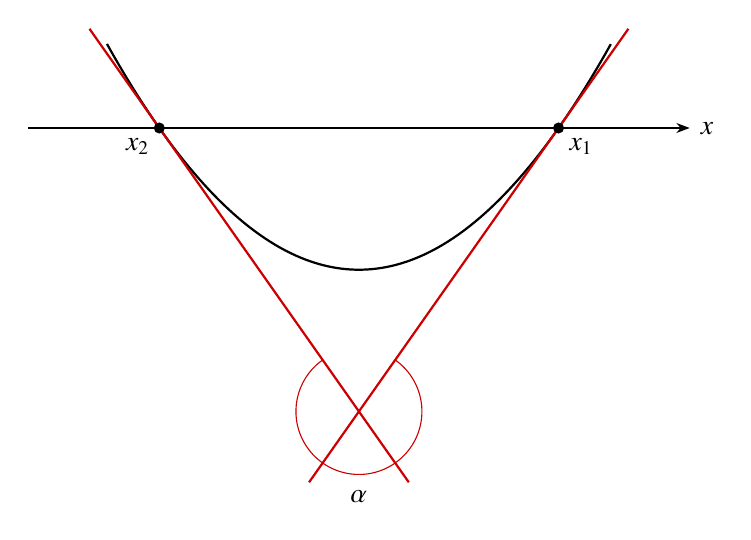
\begin{tikzpicture}[scale=1.0,>=Stealth]
\draw[->] (-4.2,0)--(4.2,0) node[right] {$x$};
\draw[thick,domain=-3.2:3.2,samples=100] plot (\x,{0.28*\x*\x-1.8});
\coordinate (L) at (-2.535,0);
\coordinate (R) at (2.535,0);
\coordinate (I) at (0,-3.6);
\draw[red!80!black,thick] ($(L)!-0.35!(I)$)--($(L)!1.25!(I)$);
\draw[red!80!black,thick] ($(R)!-0.35!(I)$)--($(R)!1.25!(I)$);
\fill (L) circle (2pt) node[below left] {$x_2$};
\fill (R) circle (2pt) node[below right] {$x_1$};
\pic[draw=red!80!black,"$\alpha$",angle radius=8mm,angle eccentricity=1.35] {angle=L--I--R};
\end{tikzpicture}
\caption{Interior angle between the tangent rays at the two real roots.}
\lb{fig:tangent_angle}
\end{figure}

If instead one chooses the oriented direction vectors $(1,\sqrt{\Delta})$ and $(1,-\sqrt{\Delta})$, the angle obtained is the supplementary angle $\theta=\pi-\alpha$, for which
\be
\cos\theta=\frac{1-\Delta}{1+\Delta}.
\ee
The sign difference is therefore geometric, not algebraic: it records which pair of rays is being used to define the angle.

Equation~\eqref{eq:tangent_angle} also gives three immediate regimes. If $0<\Delta<1$, then $\alpha$ is obtuse. If $\Delta=1$, the tangents are perpendicular. If $\Delta>1$, the marked interior angle is acute.

\subsection{Algebraic and differential viewpoints}

The vertex calculation illustrates a general principle. Completing the square is global and algebraic: it rewrites the entire function in a canonical form. Differentiation is local and analytic: it identifies the point where the slope vanishes. For quadratics, both routes are exact and elementary, so comparing them is useful. In more complicated functions a completed-square representation may not exist, while the derivative method generalizes widely. Conversely, the algebraic method works before calculus is introduced and often reveals structure that a purely procedural derivative calculation can hide.

\begin{exercise}
Find the tangent line to $f(x)=2x^2-3x-2$ at each real root and determine the angle between the two tangent rays.
\end{exercise}

\begin{exercise}
Prove directly from Eq.~\eqref{eq:tangent_angle} that the tangents are perpendicular if and only if $\Delta=1$.
\end{exercise}

%%%%%%%%%%%%%%%%%%%%%%%%%%%%%%%%%%%%%%%%%%%%%%%%%%%%%%%%%%%%%%%%%%%%%%%


\section{Applications}

Quadratic equations arise whenever a quantity depends linearly on one variable and quadratically on another, whenever constant acceleration is integrated twice in time, or whenever an optimization problem reduces to a parabola. The examples below are chosen to show how the discriminant, vertex, and factorization acquire concrete interpretations rather than merely producing numerical answers.

\subsection{The safety parabola in projectile motion}

Consider projectile motion in a uniform gravitational field with no air resistance. A projectile is launched from the origin with fixed speed $v_0$ and angle $\theta$. Eliminating time from the standard kinematic equations gives the trajectory
\be
 y=x\tan\theta-
 \frac{g x^2}{2v_0^2\cos^2\theta}.
\lb{eq:projectile}
\ee
Set $T=\tan\theta$ and use $1/\cos^2\theta=1+T^2$:
\be
 y=xT-\frac{g x^2}{2v_0^2}(1+T^2).
\ee
For a fixed point $(x,y)$, this is a quadratic equation in $T$,
\be
\frac{g x^2}{2v_0^2}T^2-xT+
\left(y+\frac{g x^2}{2v_0^2}\right)=0.
\ee
A real launch angle exists only if the discriminant of this quadratic is nonnegative. After simplification,
\be
 y\le \frac{v_0^2}{2g}-\frac{g x^2}{2v_0^2}.
\lb{eq:safety_parabola}
\ee
The boundary
\be
 y_s(x)=\frac{v_0^2}{2g}-\frac{g x^2}{2v_0^2}
\ee
is called the \emph{safety parabola}. Every point below it can be reached by at least one launch angle in the ideal model, while a point above it cannot. Points on the boundary correspond to a repeated root in $T$, meaning that exactly one launch angle reaches the point.

\begin{figure}[htbp]
\centering
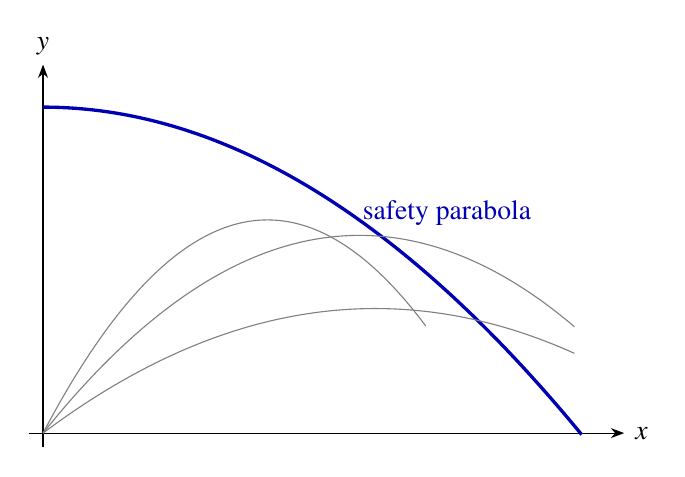
\begin{tikzpicture}[scale=0.9,>=Stealth]
\draw[->] (-0.2,0)--(8.2,0) node[right] {$x$};
\draw[->] (0,-0.2)--(0,5.2) node[above] {$y$};
\draw[very thick,blue!70!black,domain=0:7.6,samples=100] plot (\x,{4.6-0.08*\x*\x});
\draw[gray,domain=0:7.5,samples=100] plot (\x,{1.25*\x-0.14*\x*\x});
\draw[gray,domain=0:7.5,samples=100] plot (\x,{0.75*\x-0.08*\x*\x});
\draw[gray,domain=0:5.4,samples=100] plot (\x,{1.9*\x-0.30*\x*\x});
\node[blue!70!black] at (5.7,3.1) {safety parabola};
\end{tikzpicture}
\caption{The safety parabola is the envelope of projectile trajectories with fixed launch speed in the idealized uniform-gravity model.}
\lb{fig:safety_parabola}
\end{figure}

\subsection{Scalar kinematics with constant acceleration}

For one-dimensional motion with constant acceleration $a$, position is
\be
 x(t)=x_0+v_0t+\frac12at^2.
\lb{eq:kinematics}
\ee
To determine when the particle reaches a position $x=x_f$, solve
\be
\frac12at^2+v_0t+(x_0-x_f)=0.
\ee
The discriminant is
\be
\Delta_t=v_0^2-2a(x_0-x_f)
=v_0^2+2a(x_f-x_0).
\ee
The condition $\Delta_t\ge0$ determines whether the target position is reachable within the mathematical model. The two real roots, when both are physically admissible, can represent two times at which the same position is visited, for example during ascent and descent in vertical motion.

\begin{example}
A particle moves vertically according to
\be
 y(t)=20t-5t^2.
\ee
The times at which $y=15$ satisfy
\be
5t^2-20t+15=0,
\ee
so $t=1\,\mathrm{s}$ and $t=3\,\mathrm{s}$. The same height is reached once on the way up and once on the way down. The vertex occurs at $t=2\,\mathrm{s}$, where the height is maximal.
\end{example}

\subsection{Optimization problems}

Many elementary optimization problems reduce to maximizing or minimizing a quadratic. Suppose a rectangle has perimeter $P$. If one side has length $x$, the other is $P/2-x$, so the area is
\be
A(x)=x\left(\frac{P}{2}-x\right)
=-x^2+\frac{P}{2}x.
\ee
Since the leading coefficient is negative, the area is maximal at the vertex,
\be
x=\frac{P}{4}.
\ee
The other side has the same length, so among rectangles with fixed perimeter the square has maximal area. This conclusion can be obtained by completing the square or by setting $A'(x)=0$.

Quadratic optimization also appears in elementary economics. If a linear demand model makes price decrease linearly with quantity, revenue is the product of price and quantity and is therefore quadratic. The vertex then gives the revenue-maximizing quantity, subject to the limitations of the model. The mathematical procedure is simple; the modeling assumptions require more care.

\subsection{A modeling perspective}

A quadratic model should not be used merely because a parabola fits a few points. In physics, the quadratic dependence of position on time under constant acceleration follows from a dynamical assumption. In geometry, the quadratic equation follows from a locus definition. In optimization, it often follows from multiplying linear expressions. These structural derivations are stronger than curve fitting because they explain why a quadratic should appear and identify the meaning of its coefficients.

The recurring role of the discriminant is especially instructive. In pure algebra it distinguishes root types. In geometry it counts intersections. In projectile motion it separates reachable from unreachable points. In kinematics it separates attainable from unattainable events. One algebraic invariant therefore carries different interpretations without changing its mathematical definition.

\begin{exercise}
A projectile is launched from the origin with speed $v_0$. Starting from Eq.~\eqref{eq:projectile}, reproduce the derivation of the safety parabola and identify the launch angle corresponding to a point on its boundary.
\end{exercise}

\begin{exercise}
A particle has position $x(t)=4+12t-2t^2$. Determine its maximum position and the times at which it passes through $x=14$.
\end{exercise}

\begin{exercise}
A farmer has $100$ meters of fencing to enclose a rectangular region against a straight wall, so only three sides require fencing. Formulate the area as a quadratic function and determine the maximizing dimensions.
\end{exercise}


%%%%%%%%%%%%%%%%%%%%%%%%%%%%%%%%%%%%%%%%%%%%%%%%%%%%%%%%%%%%%%%%%%%%%%%
\bibliography{references}
\bibliographystyle{unsrt}

\end{document}
